% meta.concepts: dry friction
% meta.tags: realistic
% acknowledge: Peter Seiler & Luke Melander graciously shared Spring 2019 course material
% source: 2019 P. Seiler AEM2011 HW 11

Disc brakes are the most common type of brakes used in modern automobiles. They work by having a disc fixed to each wheel of the vehicle, and a hydraulic caliper which applies a force to the disc. The friction between the brake pads and the disc will slow down and ultimately stop the rotation of the wheel. 

The diagram below shows a disc brake and caliper assembly. The disc rotates about point $A$, and when the brakes are actuated, a force of $-N {\bf k}$ (into the page) is applied to the front of the disc, and a force of $+N {\bf k}$ (out of the page) is applied to the back of the disc. Both forces act at point $B$, which is given by $-10 {\bf i} + 3 {\bf j}$ centimeters. The coefficients of friction between the brake pads and disc are $\mu_s = 0.5$ and $\mu_k= 0.4$.

\begin{enumerate}
  \item When the brakes are fully actuated, the force $N$ reaches its maximum value of $20kN$. If the car is at rest and the brakes are fully actuated, what is the maximum moment that can be supplied by the axle before the brakes fail and the car begins to move?
  \item When the car is coasting down a steep hill, a moment of $200$ $N\cdot m$ is generated about the axle. If light brake pressure is applied, the car will move down the hill at a constant speed instead of accelerating. What is the force $N$ that the brakes must apply for the car to move at a constant speed?
\end{enumerate}

\begin{figure}[ht!]
  \centering
  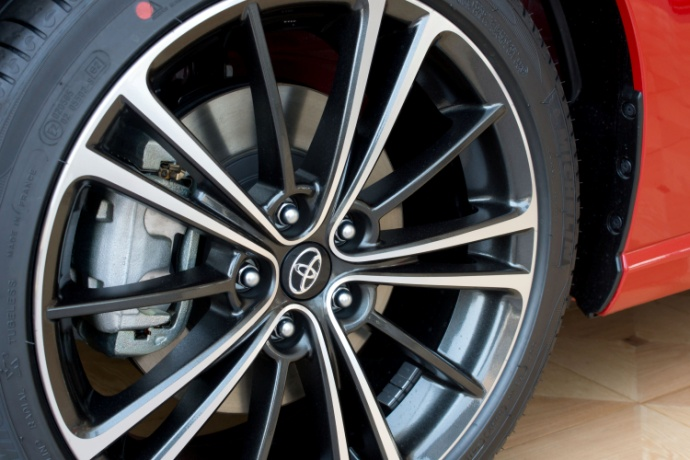
\includegraphics[width=0.4\textwidth,
	           height=0.1\textheight,
		   keepaspectratio]{figa.png}
  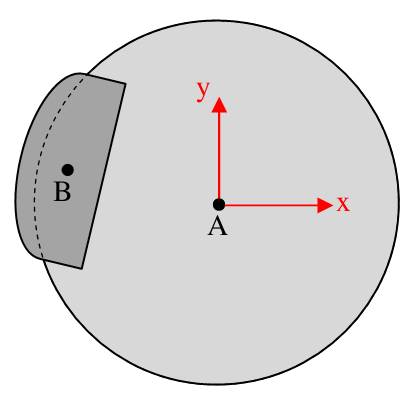
\includegraphics[width=0.4\textwidth,
	           height=0.1\textheight,
		   keepaspectratio]{figb.png}
\end{figure}

\iftoggle{flagSoln}{%
\vspace{.5cm}
\rule{\textwidth}{.4pt}
\vspace{.5cm}
\textbf{Solution:}
\begin{figure}[ht!]
  \centering
  \frame{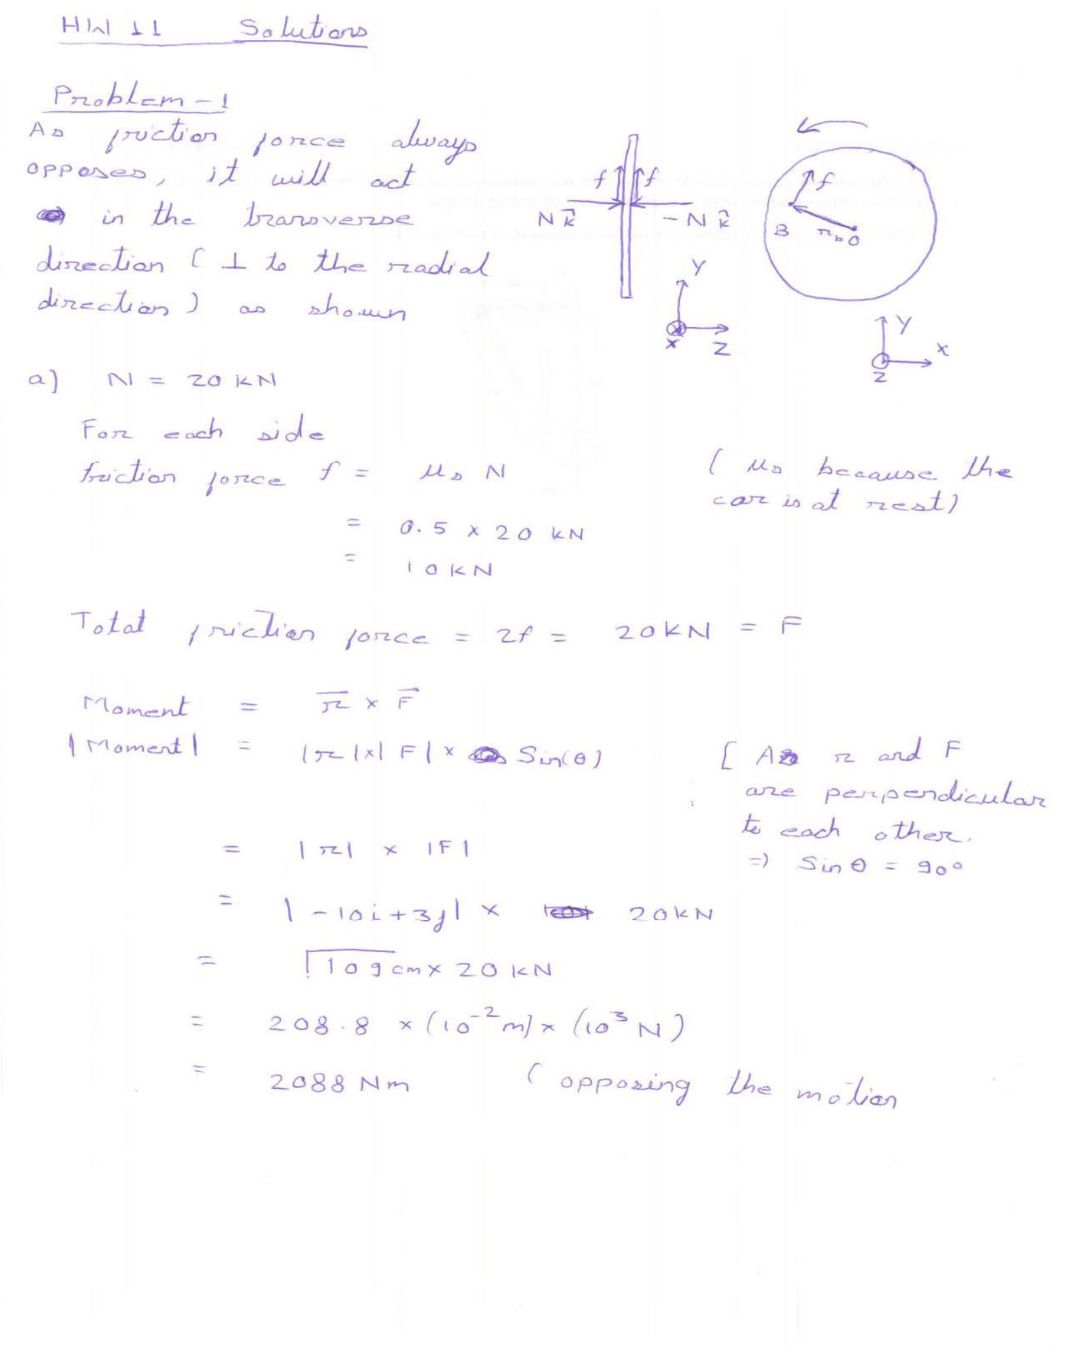
\includegraphics[width=0.9\textwidth,
	           height=0.4\textheight,
       keepaspectratio]{solna.png}}
  \frame{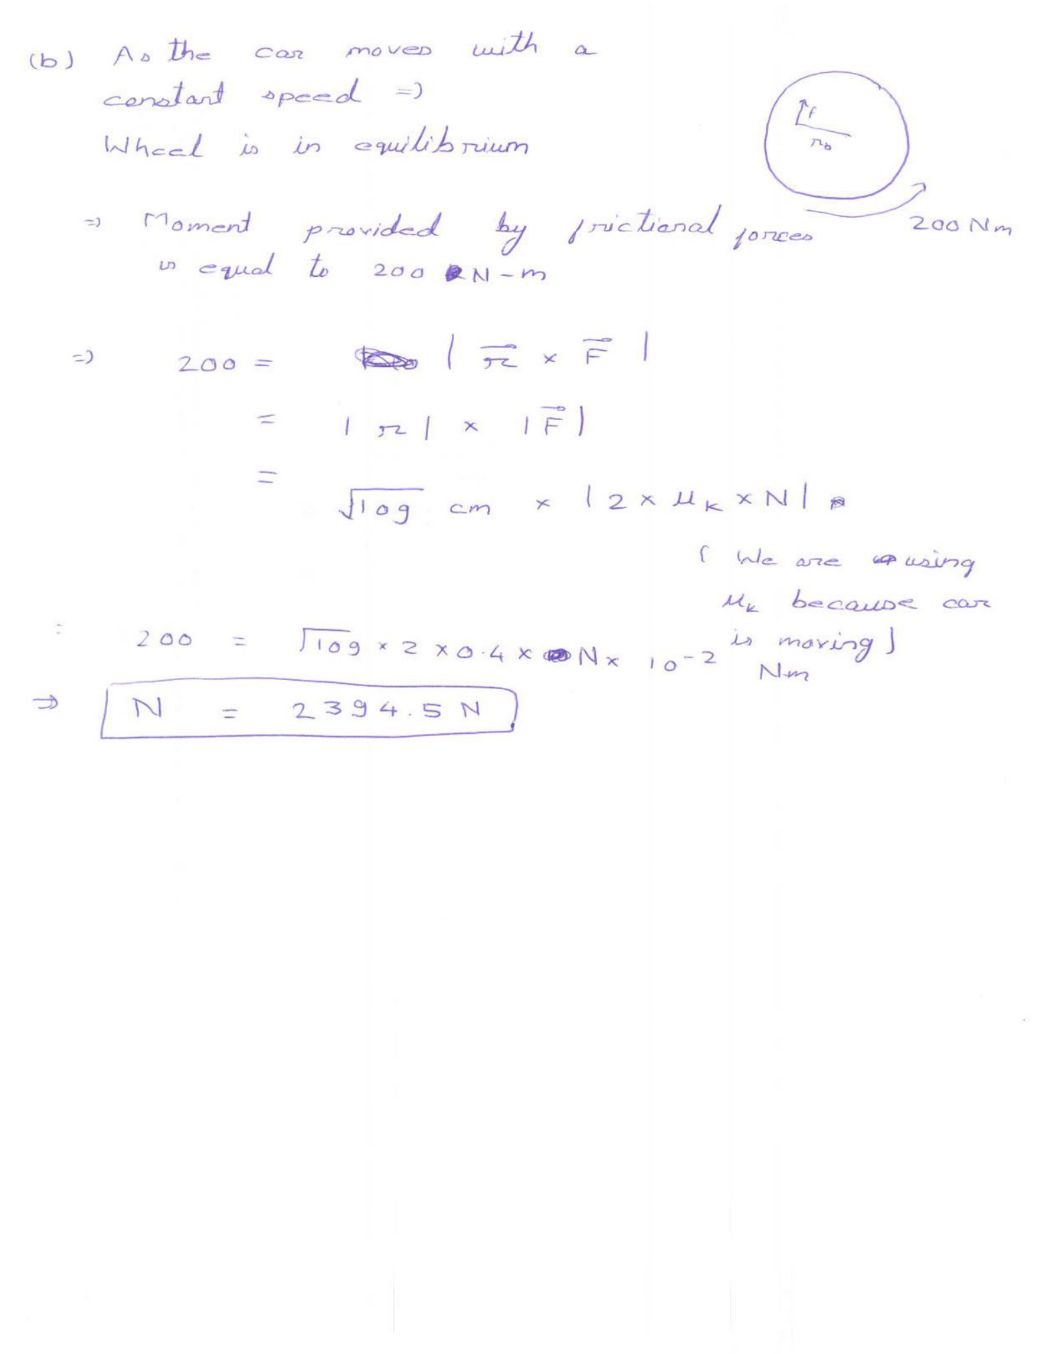
\includegraphics[width=0.9\textwidth,
	           height=0.4\textheight,
       keepaspectratio]{solnb.png}}
\end{figure}
}{%
}%
